\chapter{Background}


In this chapter will introduce all the background that is helpful to understand this Bachelor's thesis. 
First off, it will explain what the USB protocol is and how it works, next the kind of attack this thesis deals with, and finally the hardware that is involved, specifically the O.MG cable. 

\section{The USB Protocol} \label{TheUSBProtocol}

The USB standard \cite{WaybackMachine2018} was first published in 1996. It was developed in a collaboration between the tech companies Compaq, DEC, IBM, Intel, Microsoft, NEC, and Nortel as a new standard to connect slow peripheral devices. To this end, they founded a new non-profit, called the USB Implementation Forum \cite{USBIFUSBIF}. It's goals were:
\begin{itemize}
    \item "Ease of use for PC peripheral expansion"
    \item "Low-cost solution that supports transfer rates up to 12 Mbs"
    \item "Full support for the real-time data for voice, audio, and compressed video"
    \item "Protocol flexibility for mixed-mode isochronous data transfers and asynchronous messaging"
    \item "Integration in commodity device technology"
    \item "Comprehend various PC configurations and form factors"
    \item "Provide a standard interface capable of quick diffusion into product"
    \item "Enable new classes of devices that augment the PC's capability"  
\end{itemize}
\cite[p.~23]{WaybackMachine2018}\\
The creators wanted to create an universally applicable standard protocol, for all sorts of data connections, that is also flexible, and on top of all that easy to use and low in cost. Their solution was the Universal Serial Bus.

\begin{figure}
    \centering
    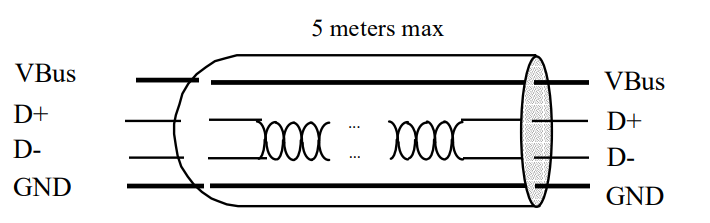
\includegraphics[width=0.5\linewidth]{usbsingalgraphic.png}
    \caption{USB Cable Signals}
    \label{fig:usbsingalgraphic}
    \cite{WaybackMachine2018}
\end{figure}

In figure \ref{fig:usbsingalgraphic} we can see how a USB cable is constructed. \\
The connection is built upon four signal lines; a negative (Ground) powerline GND, a positive powerline VBUS for the power supply, and two data transfer lines D+ and D-. The two physical transfer data lines are aligned as a twisted pair. This alignment protects them from outside electrical noise and does not mean that more than one logical line is available. They work together to transmit one logical signal, one single bit. USB utilizes Non Return to Zero Inverted (NRZI) meaning that the bits on the bus are represented by a transition of physical levels, rather than the presence or absence of them. A powerchange during a time interval signals a 1, if the connection stays constant, it's a 0. This allows data transfer while simultaneously allowing the participating parties to synchronise their bit clocks.  \\
Since there is only one logical data line, data transfer can only happen in one direction at a time. Bi-directional communication happens in half-duplex mode; the parties alternate. To deal with this restriction, a protocol that manages data and sender order has to be followed; the USB protocol.  

This next section will expand on the functionalities of the USB protocol as described by \cite{nissimUSBbasedAttacks2017}. 

A USB connection includes a host, usually a computer, and one to many peripheral devices that connect to the PC's embedded USB hub.  \\
USB devices generally fit into two categories; I/O devices that add capabilities to the host, and hub devices which connect additional devices to the host. An USB cable has two main functionalities; Establishing a data connection to allow communication between the connected parties, and supplying electrical power to the connected peripheral device if it is not self-powered. Such devices that draw power from an USB Host are called bus-powered. \\ 
For bus-powered devices it is important to receive the power from the UBS cable before it is supposed to process any data, which is why the USB connector was specifically designed with power pins that are longer than the signal pins.\\
Every USB device is equipped with a microcontroller chip that manages the USB interactions with the host, and optionally also has a bootloader that allows loading firmware, for example for updates. \\
One USB device consists of one to multiple logical subdevices that are known as device functions. For a webcam with built in audio this would correspond to a video and an audio function. Devices with multiple subdevices are referred to as composite devices. Each functions is managed through a separate endpoint on the bus with it's own logical address. One endpoint forms a logical communication channel called a pipe, of which there are two types.  
\begin{enumerate}
    \item Message Pipe: A message pipe is used for control transfers. That means they are used for short and simple commands sent to the USB device and status responses to the host.
    \item Stream Pipe: A stream pipe is used for actual data transfer.
\end{enumerate}
Data transfer can only take place if the host directly requests it. An USB device cannot transfer information autonomously. 

In order to be able to communicate with any USB device, a connection needs to be established and initialized. This is done with a process called 'enumeration' that starts as soon as the physical connection is established. It consists of four main steps;

\begin{enumerate}
    \item \emph{Detection}: A change in the current on the data lines is detected by the host, so it knows that a new USB device has been connected.
    \item \emph{Device Speed}: The speed of the device is determined by using the change on  the data lines in step 1.
    \item \emph{Device Descriptors}: The USB device is reset by the host through a specific dataline signal. This prompts the device to send information about itself (it's descriptors) to the host by which it is identified.  \\
    The exchange of descriptors follows a defined order; 
    \begin{itemize}
        \item First the host will request the descriptor length and the descriptor from the device with the Get\_Device\_Descriptor command.
        \item The advice is reset again and given a unique local address by the host called via the Set\_Address command. 
        \item Lastly, the device is prompted to send it's configuration by the Get\_Configuration\_Descriptor. The configuration includes a hierarchy of interface, endpoint and class specific descriptors.  
    \end{itemize}
    \item \emph{Loading Drivers}: Now that all the information has been exchanged the host can start using it to load the device specific driver's that will allow it to be controlled. The corresponding driver is found by the USB class, the vendor ID (VID) and the product ID (PID). Most standard drivers are included in the OS of the host, if they aren't the user has to download them manually. This concludes the enumeration process, after these steps the device is ready for use.
\end{enumerate}




\section{The Dangers of USB} \label{TheDangersOfUSB}

Some people might notice that during the initialization process described in section \ref{TheUSBProtocol} there are no verification or authorization steps. The protocol assumes that any physically connected USB device is trustworthy and does not take any precautions to check its claims and properties. \\
This is a big oversight and opens the door for a lot of malicious activity. 
The risks posed by this activity is exacerbated by the fact that USB devices are not perceived as a threat by a vast majority of people. In fact, many would absolutely pick up, plug in, and even interact with USB sticks they find lying around on the ground. A study \cite{tischerUsersReallyPlug2016} conducted in 2016 found that USB sticks are a very effective attack vector. They explored whether USB sticks dropped on a university campus would really be picked up and plugged in. They found that users opened one or more files on 45\% of the flash drive and that 98\% of the drives were removed from the drop location by the time the experiment had ended. Based on this, the authors estimate that between 45\% and 98\% of drives were eventually plugged in. On the drives the authors placed information for a survey to explore the finder's motivation. From this survey it was concluded that the USB drives were plugged in mostly out of altruistic motives (to find the owner). The social engineering attack was an "expeditious" vector with a median time of connection of only 6.9 hours.  \\
USB ports are common also in public, for convenient charging on the go, for example in Buses or Airports \cite{kumarJuiceJackingUSB2020}. People rarely think twice when they connect their laptop to an external display in a library or accept a charging cable from a friend. None of these actions are protected, and every interaction through the USB protocol poses a risk most are not aware of.

A myriad of different attacks are possible through such an unsecured attack vector.\\
Through USB, data can be silently downloaded without the user's permission or knowledge from computers \cite{clarkHardwareTrojanHorse2009} as well as phones \cite{SharpIdeasDownloads2006}. USB drives developed to be able to do data manipulation, and with the increased popularity of U3, attackers could hack U3 images and replace them for their own malicious purposes to take advantage of auto-run. 
How much damage could be done with this is best exemplified with Stuxnet \cite{kushnerRealStoryStuxnet2013}. It's a malware program that could travel via USB; a computer that came in contact with an infected USB stick would immediately be compromised. In this way, malware could spread even in an air-gaped environment. The highly sophisticated and targeted attack was discovered in 2010 and is confirmed to have damaged centrifuges that were part of Iran's Nuclear Program.\\
But an attack via USB does not have to have the dimensions of an (alleged) geopolitical intelligence mission \cite{kushnerRealStoryStuxnet2013}, there are more examples of day-to-day threats to exemplify what USB can do. On Windows XP it is possible to emulate a CD-ROM device through an USB connection and hack the U3 autoplay feature \cite{al-zarouniRealityRisksConsented2006}, data can be exfiltrate from iOS6 through a USB charging cable \cite{lauMactansInjectingMalware2013}, USB can be used to propagate attacks from one computer to another, as demonstrated in \cite{wangExploitingSmartphoneUSB2010}, or destroy a target with power surges that irreparably damage the host \cite{USBKillDevices}, Fork Bomb attacks can be launched via USB \cite{efendyExploringPossibilityUSB2019}, and, most importantly, since USB does not require authentication, it can be used to emulate other devices, namely devices that are used for human input. Human Interface Devices (HID) such as keyboards and mice present an unparalleled attack vector, where a hacker with physical access to an unlocked computer can remotely execute any action a user themselves could \cite{USBRubberDucky}, \cite{MGCable2019a}, \cite{lawalFacilitatingCyberenabledFraud2022}. \\
How such HID attacks could look like, and the extent their damage can reach, will be discussed and exemplified in section \ref{Methodology}.

\subsection{Bad Hardware}

None of the attacks and only part of the defenses that are discussed in this thesis would be possible without specialized hardware. This section will therefore give a brief introduction into the different microcontrollers and computers that will be mentioned in the following chapters.\\
In general, any USB deivce that has been modified to execute some malicious action will be referred to as BadUSB, a term coined by a BalckHat presentation by Karsten Nohl, Sascha Krissler, and Jakob Lell \cite{Srlabsbadusbblackhatv1Pdf2014}. 


\subsubsection{Arduino}

\begin{figure}[H]
    \centering
    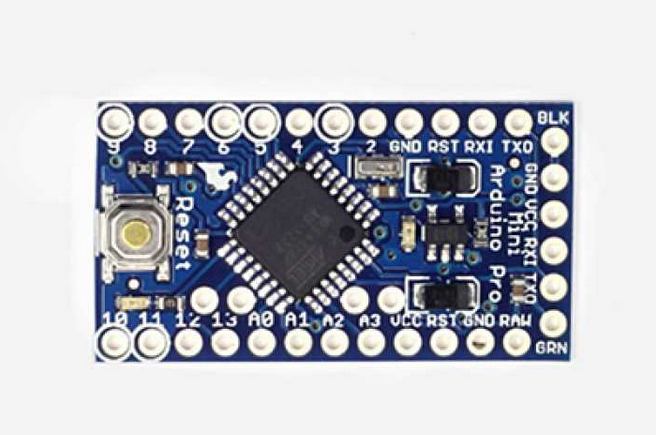
\includegraphics[width=0.25\linewidth]{arduinomini.png}
    \caption{The Arduino pro mini, used by \cite{bojovicRisingThreatHardware2019}}
    \label{fig:ArduinoProMini}
    \cite{ArduinoProMini}
\end{figure}
Arduino \cite{ArduinoHardware} is a company that produces a range of different small microcontrollers designed to be accessible and straight forward. They are supported by the open-source Arduino platform and the Arduino IDE \cite{ArduinoArduino2024}.


\subsubsection{Teensy}

\begin{figure}[H]
    \centering
    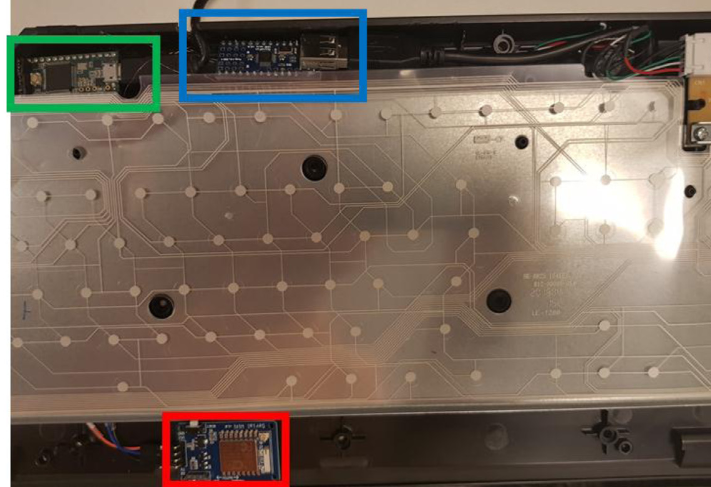
\includegraphics[width=0.5\linewidth]{teensy.png}
    \caption{Teensy (in green) as built into Malboard}
    \label{fig:builtInTeensy}
    \cite{farhiMalboardNovelUser2019}
\end{figure}

The Teensy  \cite{TeensyUSBDevelopment} is a microcontroller system based on USB, that is, as it's name suggests, tiny. It can be programmed via it's USB port, is compatible with Arduino Software and works with Mac OS, Linux, and Windows. It comes standard with solder pads. To program it, the Teensy Loader Application can be used.
A teensy can be programmed to emulate a keyboard and a mouse and change its PID and VID \cite{farhiMalboardNovelUser2019}.\\
These qualities, especially it's size, make it a popular microcontroller for self made BadUSBs. 


\subsubsection{Hak5 Hardware} \label{Hak5Hardware}

\begin{figure}[H]
    \centering
    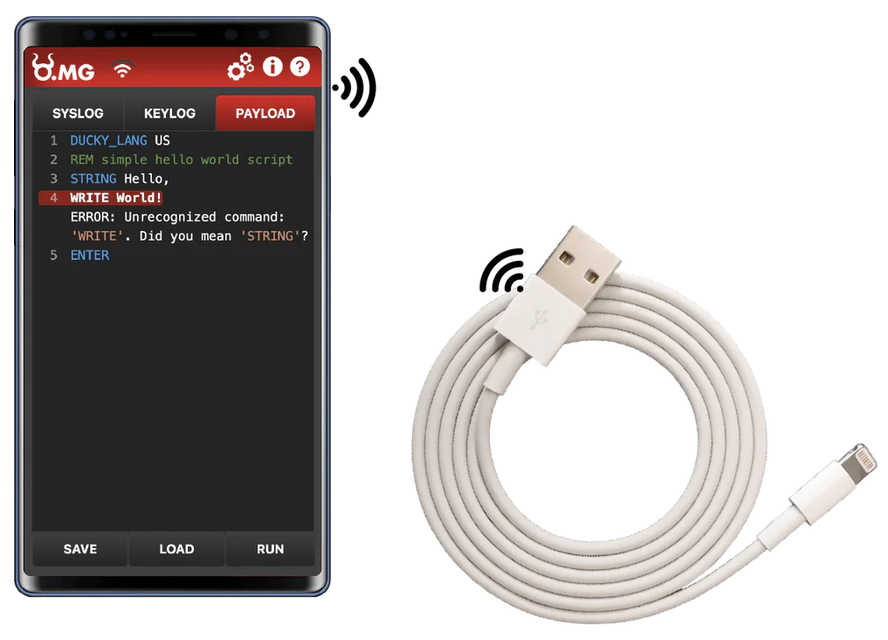
\includegraphics[width=0.5\linewidth]{OMGCable.png}
    \caption{The O.MG cable and it's Web IDE open on a phone}
    \label{fig:OMGCable}
    \cite{hak5MGCable}
\end{figure}

Hak5 is a company founded in 2005 by who have made it their missions to 'advance the InfoSec industry' \cite{hak5}. They have an award winning podcast, a big YouTube channel, and a lot of penetration testing gear. They aim to inform people of the security risks that come with tech with the goal of ultimately making the world a safer place. \\
In 2019, the O.MG cable was made available at Hak5 \cite{MGCable2019a} marking the beginning of a collaboration between the creator of the O.MG cable and founder of Mischief Gadgets, MG \footnote{https://twitter.com/_MG_} and the Hak5 team. They have since released many variations of the O.MG cable, including a plug, an adapter, an 'unblocker', and a cable detector \cite{hak5MischiefGadgets}. The device that will be featured in this thesis is the O.MG cable. It is essentially plug and play and can therefore be used to conduct injection attacks, without having to do any hardware building yourself \cite{hak5MGCable}. 



\section{DuckyScript and the O.MG cable}


This section will give an overview over the O.MG cable, and the scripting language it is equipped with; DuckyScript. 

\subsection{The O.MG cable} \label{theOMGCable}

As described shortly in sections \ref{Hak5Hardware} and \ref{HistoryOfAttacks} the O.MG cable is a BadUSB cable invented by MG \cite{MGCable2019a}, produced by Mischief Gadgets \cite{hak5MischiefGadgets} and sold in cooperation with Hak5 on their website \cite{hak5MischiefGadgets}. \\
The cable does not have any physical markers; neither it's USB ends, the cable, nor the weight gives any indication that it has so many more capabilities than other USB cables. For the most part, it is a usual USB cable; the non-active (passthrough) end does not have any special abilities, and if it is not configured to execute a boot script, the cable can be used like any other to charge an transfer data. It's malicious active end is marked by a USB trident as found often on USB cables to indicate their compatibility with the USB standard. That end transmits the payloads on the device to the USB host. It is available in USB-A, USB-C and lightning. 
When setting up to use a O.MG cable ,the very first thing that has to be done is flashing it. The cable has to be flashed before it is used, or after a self-destruct was triggered. To flash it, a O.MG Programmer is needed \cite{hak5MGCable}. The active end of the O.MG cable is plugged into the programmer, which itself is connected to a computer by a regular USB data cable. Flashing can either be done with the official open source firmware \cite{DuckyScriptSyntaxGuide} via the website \footnote{https://o.mg.lol/setup/OMGCable/} or with custom firmware. \\  
Once the device has been flashed, it is ready to be used. Once an active end received power from a USB host, it established a small Wifi network, with the default SSID O.MG and password 12345678, both of which can be changed. Through that network the WebUI to control the cable can be accessed via http://192.168.4.1 . \\
The WebUI offers a lot of different features [TODO; add screenshot of the webUI]

\begin{enumerate}
    \item Payloads
    \item Geofencing
    \item Self-Destruct
    \item Keymap Viewer
    \item Keylogger
    \item Partition Editor
    \item C2
    \item HIDX StealthLink
\end{enumerate}

The following subsections contain a short description of each of these features. 

\subsubsection{Payloads}

All O.MG devices that can be programmed for keyboard injection support an enhanced version of DuckyScript. Basic Duckyscript, as expanded upon in section \ref{DuckyScript} does not support all the extra features of the O.MG devices, such as self-destruct or GeoFencing. \\
Payloads can be written directly in the WebUI, where they can be stored into slots. Depending on the model, the cable supports from 8-200 payload slots \cite{hak5MGCable}. They can be directly executed via the WebUI (executed on the host connected to the active end), stored on the cable, modified, and accessed, or set as a bootscript. Only one payload can be a bootscript; it is a script that is executed as soon as the active end is connected. \\



\subsubsection{Geofencing}

Geofencing can be accomplished by a simple conditional statement. With it is possible to trigger or block actions depending on the presence or absence of a wifi network with a specific SSID. This is accomplished by a condition that is evaluated every time the O.MG device powers up. Alternatively, the cable can wait until a SSID or BSSID is present with the 'WAIT\_FOR\_PRESENT' keyword.
It will either wait for a specific amount of time or run forever. Conversely, this feature can also be used to wait until out of reach of a network.

\subsubsection{Self-Destruct}

Cleanup is an important part of an attack or penetration test. This cable supports two kinds of self-destruct that can be triggered via the WebUI or with a keyword in the code.
\begin{itemize}
    \item  \textbf{Self-Destruct 1:} Completely erases all data on the cable and disconnects the data line. The cable will appear broken. To use it again, it has to be physically recovered and reflashed.  
    \item  \textbf{Self-Destruct 2:}  Erases all the data but retains the data lines, turning the cable in a normal USB cable. Reflashing is also necessary to use the cable again. 
\end{itemize}


\subsubsection{Keymap Viewer}

Since the O.MG cable imitates keyboard presses, it is dependent on the keyboard settings of the attacked host. Input in a US keyboard will not produce the same signal to the computer as a DE\_CH keyboard even though the same key is pressed. For this reason, the lanugage of a payload has to be set, which is explained in more detail in section (TODO!!). If the keyboard settings of the target are not known beforehand, obtaining this information in the reconnaissance phase is crucial. \\
For this reason the Keymap Viewer exists. Through the WebUI the keyboard layout of a connected host can be determined. (TODO; try this out!!)

\subsubsection{Keylogger}

When an O.MG cable is connecting a physical keyboard with a detachable cable to a host, it can keylog the strokes from the keyboard and display them in real time on the WebUI. In order for this to work, the keyboard has to be Full Speed USB (12mbps) and not low (1.5mbps) or high speed (480mbps) 

\subsubsection{Partition Editor}

On specific models of the O.MG cable a user can device themselves how the available storage should be used with the partition editor. They can decide to redirect storage resources to payload slots, individual slot size, size of storage for exfiltrated data, or keylogging storage. 

\subsubsection{C2}
A C2 server eliminates the need for physical proximity to the O.MG device to connect to and communicate with it. The cable can connect to the C2 server as well as the attacker. This way it can be controlled from anywhere. 

\subsubsection{HIDX Stealth Link}
This feature is still in progress, but the idea is to enable more stealthy data exfiltration. Instead of establishing a network or sending the data via the host, the cable relays the data via the HID channels.  


\subsection{Ducky Script} \label{DuckyScript}

DuckyScript was invented by Darren Kitchen, the founder of Hak5. It evolved from a macro scripting language that could handle keyboard injections and delays in it's first iteration to a structured and feature rich programming language supporting injection attack specific commands (jitter, side-channel exfiltration) as well as control flow instructions, repetitions and functions in version 3.0. \cite{the book} [TODO cite the book!!] \\
Some specific Hak5 gear like the BashBunny or LANTurtle use an interpreted version of DuckyScript 1.0 that couples the BASH shell scripting language. \cite{Hak5Usbrubberduckypayloads2024} The DuckyScript version licenced for the O.MG cable is based on DuckyScript 1.0 and additionally includes some device specific commands for the specific functionalities of the O.MG cable. The available DuckyScript 1.0 commads are limited to REM (marks a comment), DELAY (pauses the payload), STRING (injects keystrokes) and some buttons like ENTER, GUI, F11, PAGEUP, TAB; ESCAPE etc. \\
A basic implementation of a Hello, World! Program for the O.MG cable could look like this:

\begin{verbatim}
REM Title: Hello, World!
REM Description: Write Hello, World! in the terminal
REM Target: Windows (including Powershell 2.0 or above)

DELAY 3000
GUI r
DELAY 750
STRING cmd
ENTER
DELAY 2000
STRING Hello, World!
\end{verbatim}



\section{Chapter Conclusion}

This chapter introduced the USB standard and protocol and the vulnerabilities that come with it. \\
It explained, how the lack of USB authentication can be leveraged by malicious actors to target users, in a stealthy and efficient way. 
Lastly, a basic overview over the hardware in this thesis was given and the O.MG cable, as well as it's scripting language, DuckyScript was introduced. 